%%%%%%%%%%%%%%%%%%%%%%%%%%%%%%%%%%%%%%%%%%%
%\subsection{Описание предметной области}
\subsection{Пример процесса проектирования некоторого технического устройства}
%%%%%%%%%%%%%%%%%%%%%%%%%%%%%%%%%%%%%%%%%%%
\begin{frame}%[allowframebreaks=0.9,t]
Дана задача -- спроектировать технический объект. Как это сделать?

В качестве технического объекта рассмотрим радиоуправляемого робота с пилой на подвижном манипуляторе.
\begin{figure}[!ht]
  \begin{minipage}{0.455\linewidth}
    В его конструкции можно выделить следующие элементы:
    \begin{itemize}
      \smaller[1]
      \arrowitem{бронированный корпус};
      \arrowitem{манипулятор};
      \arrowitem{пила};
      \arrowitem{колёса};
      \arrowitem{двигатели};
      \arrowitem{привод пилы};
      \arrowitem{привод колёс};
      \arrowitem{батарейный отсек};
      \arrowitem{радио-электронные компоненты};
      \arrowitem{\ldots}
    \end{itemize}
  \end{minipage}%
  \begin{minipage}{0.455\linewidth}
    \centering
    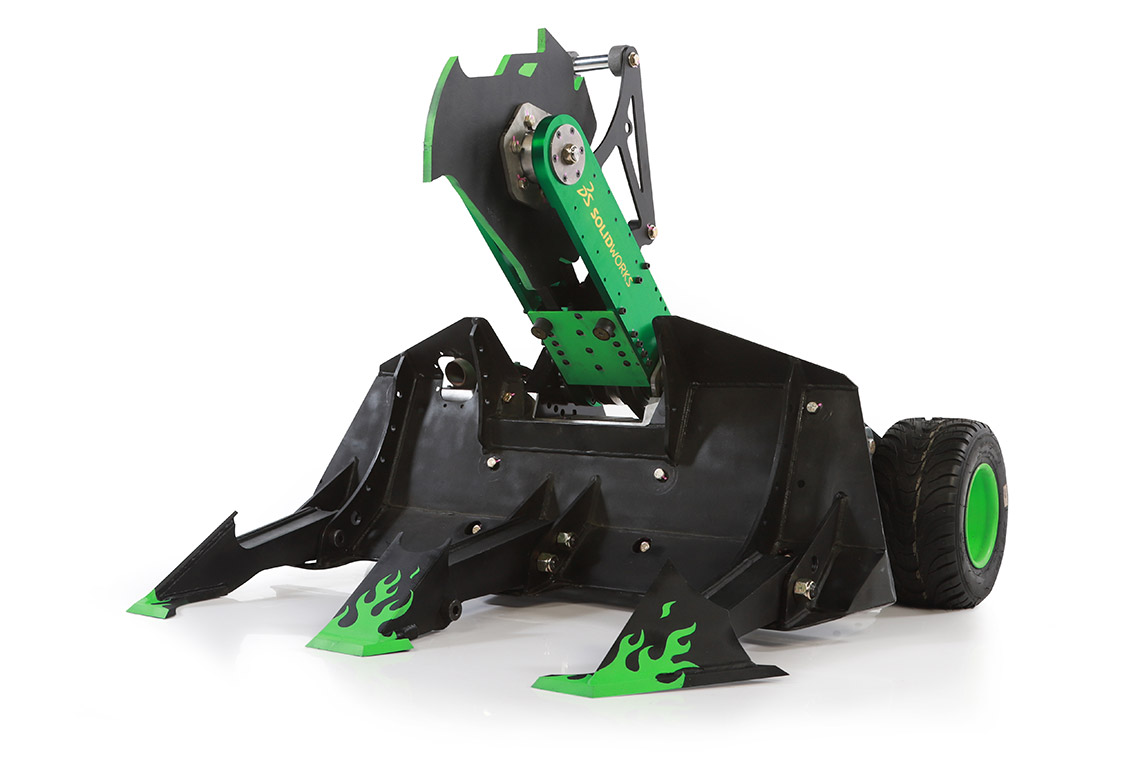
\includegraphics[width=\textwidth]{images/robot.jpg}
    \caption{Пример проектируемого объекта}
    \label{fig:technicalObjectExample}
  \end{minipage}
\end{figure}

%\onslide<1->{
%\begin{center}
%  \begin{tikzpicture}
%   \draw (0,0) -- (10,0) -- (10,3) -- (0,3) -- (0,0);
%   \end{tikzpicture}
%\end{center}}

\end{frame}
%%%%%%%%%%%%%%%%%%%%%%%%%%%%%%%%%%%%%%%%%%%
\begin{frame}[t]
	%{
    \smaller[1]
    \only<1>{%
    \begin{itemize}	
      \item Перед началом проектирования формулируется техническое задание.
      \item В начале целесообразно проектировать элементы конструкции, не зависящие от других.
    \end{itemize}
	  }
    
    \only<2>{%
    \begin{itemize}	
      \item Затем проектируются элементы конструкции, конфигурация которых зависит от других.
      \item Параметрами проектирования подобных элементов являются характеристики других (геометрические, кинематические, мощностные и проч.)
    \end{itemize}
    }

    \only<3, 4>{%
    \begin{itemize}	
      \item Затем проектируются подсистемы, объединяющие в себе различные элементы, сборочные узлы.
      \item Кроме того, проектируются элементы, которые должны содержать в себе другие сборочные узлы (корпуса и т.п.).
    \end{itemize}
    }

    \only<5>
	
	\begin{figure}[!ht]
    \centering
		\only<1>{%
		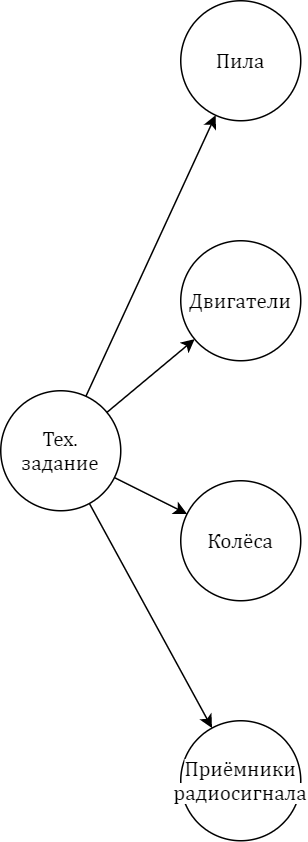
\includegraphics[scale=0.17]{images/design.frame02.png}
		}
		\only<2>{%
		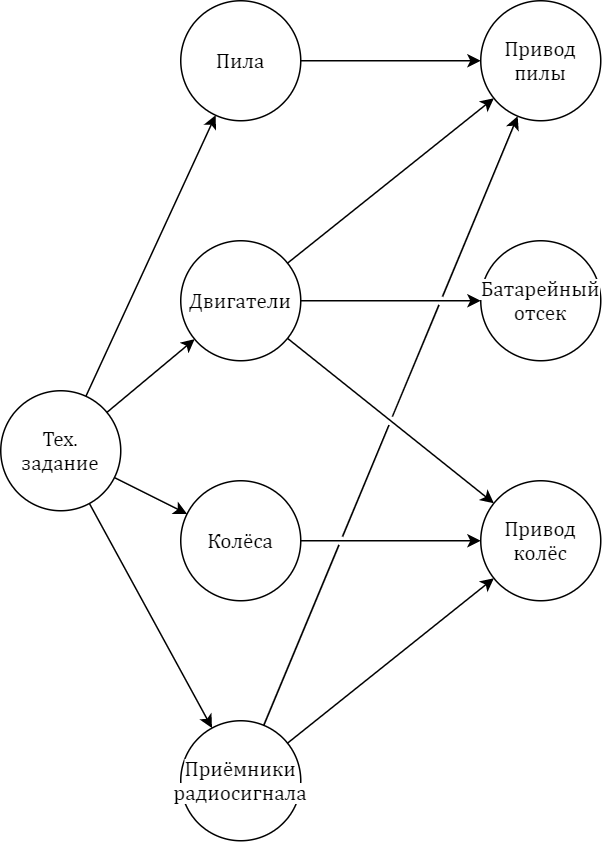
\includegraphics[scale=0.17]{images/design.frame03.png}
		}
		\only<3>{%
		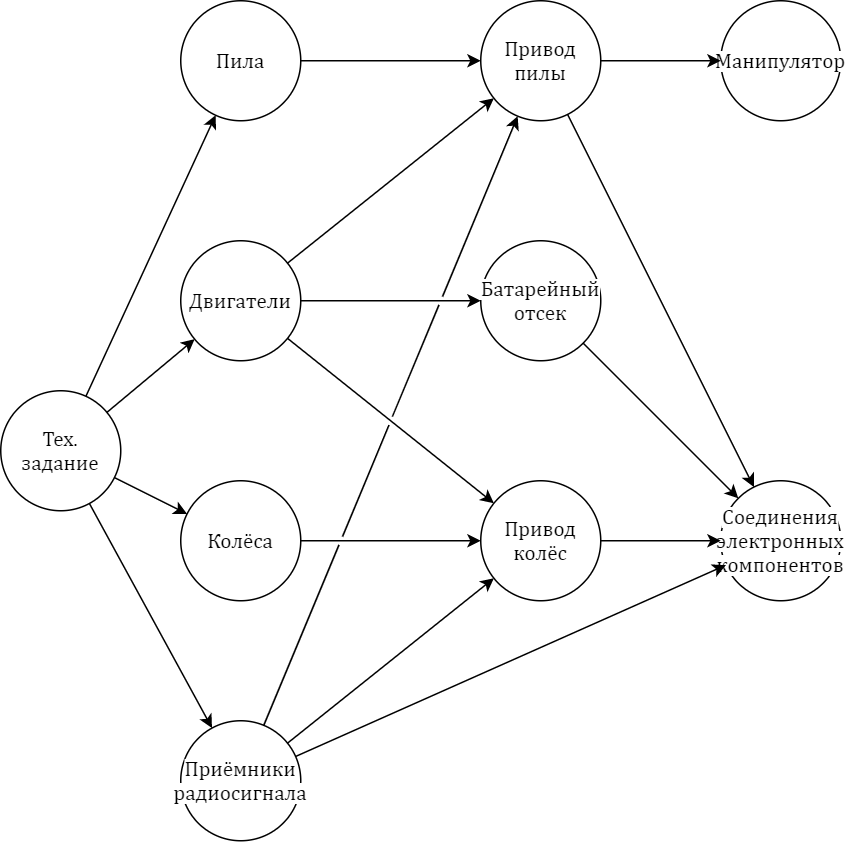
\includegraphics[scale=0.17]{images/design.frame04.png}
		}
		\only<4, 5>{%
		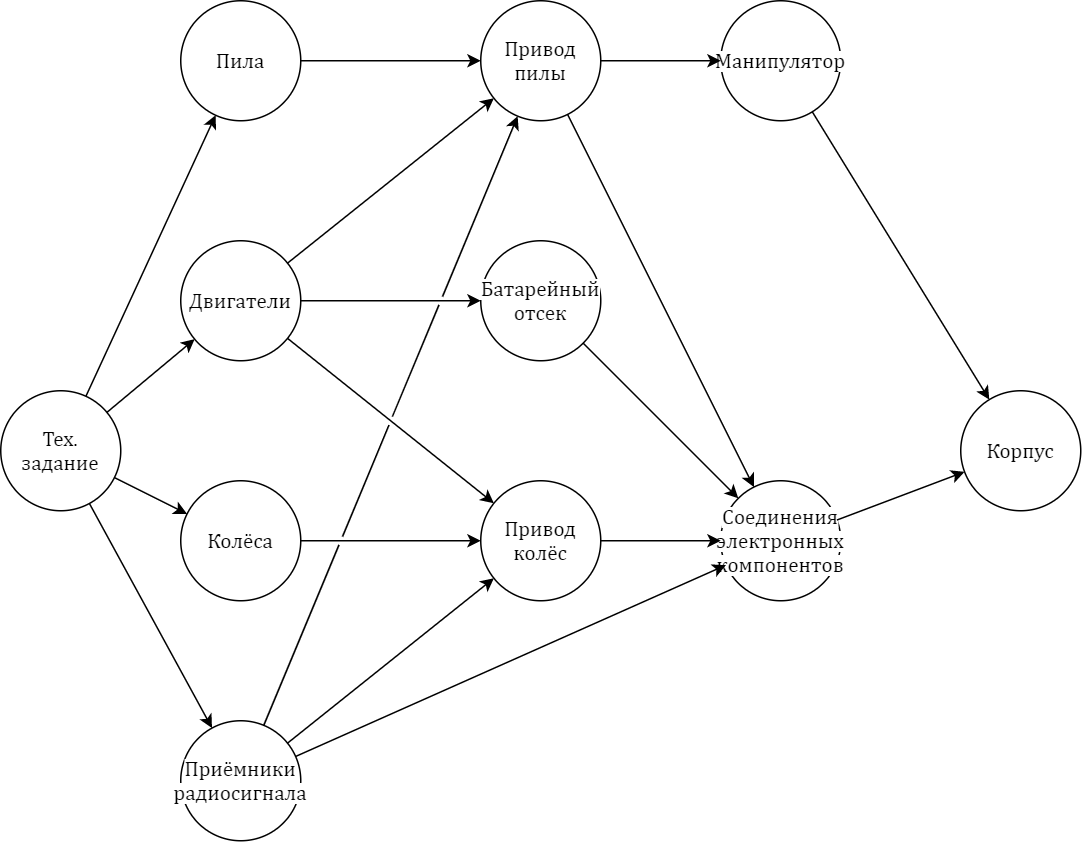
\includegraphics[scale=0.17]{images/design.frame05.png}
		}
		\caption{Проектирование мобильного робота по компонентам}\label{fig:desgin.graph}
  \end{figure}

\end{frame}

%%%%%%%%%%%%%%%%%%%%%%%%%%%%%%%%%%%%%%%%%%%
\subsection{Возможные формы представления процесса проектирования}
%%%%%%%%%%%%%%%%%%%%%%%%%%%%%%%%%%%%%%%%%%%
\begin{frame}
  \emph{Графоориентированный подход} -- подход к описанию процесса решения сложной вычислительной задачи, при котором отдельные вычислительные процессы выстраиваются в ориентированный граф.

  \begin{figure}[!ht]
    \centering
    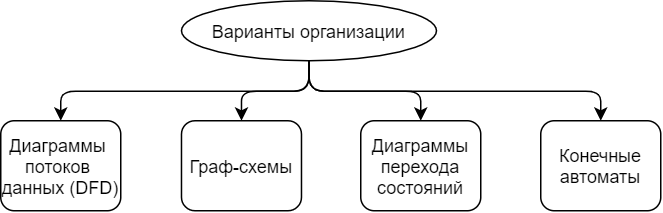
\includegraphics[width=0.6\textwidth]{images/design_graph_variants.png}
    \caption{Различные формы организации процессов проектирования в виде графа\footcite{SokolovCADCMInteraction2021}}
    \label{fig:designGraphVariants}
  \end{figure}

  В данной работе внимание сосредоточено на подходе, реализованном в разработанном Соколовым~А.П. и Першиным~А.Ю. графоориентированном программном каркасе GBSE.
\end{frame}

%%%%%%%%%%%%%%%%%%%%%%%%%%%%%%%%%%%%%%%%%%%
\subsection{Методология графоориентированного подхода (GBSE)}
%%%%%%%%%%%%%%%%%%%%%%%%%%%%%%%%%%%%%%%%%%%
\begin{frame}
  В основе описываемого подхода следующие утверждения:
  \begin{itemize}
    \item Узлу ориентированного графа соответствует \emph{состояние данных} -- некоторый строго определённый набор именованных переменных фиксированного типа, характерных для решаемой задачи;
    \item Ребру ориентированного графа соответствует процесс преобразования одного состояния данных в другое.
  \end{itemize}

  \begin{figure}
    \centering
    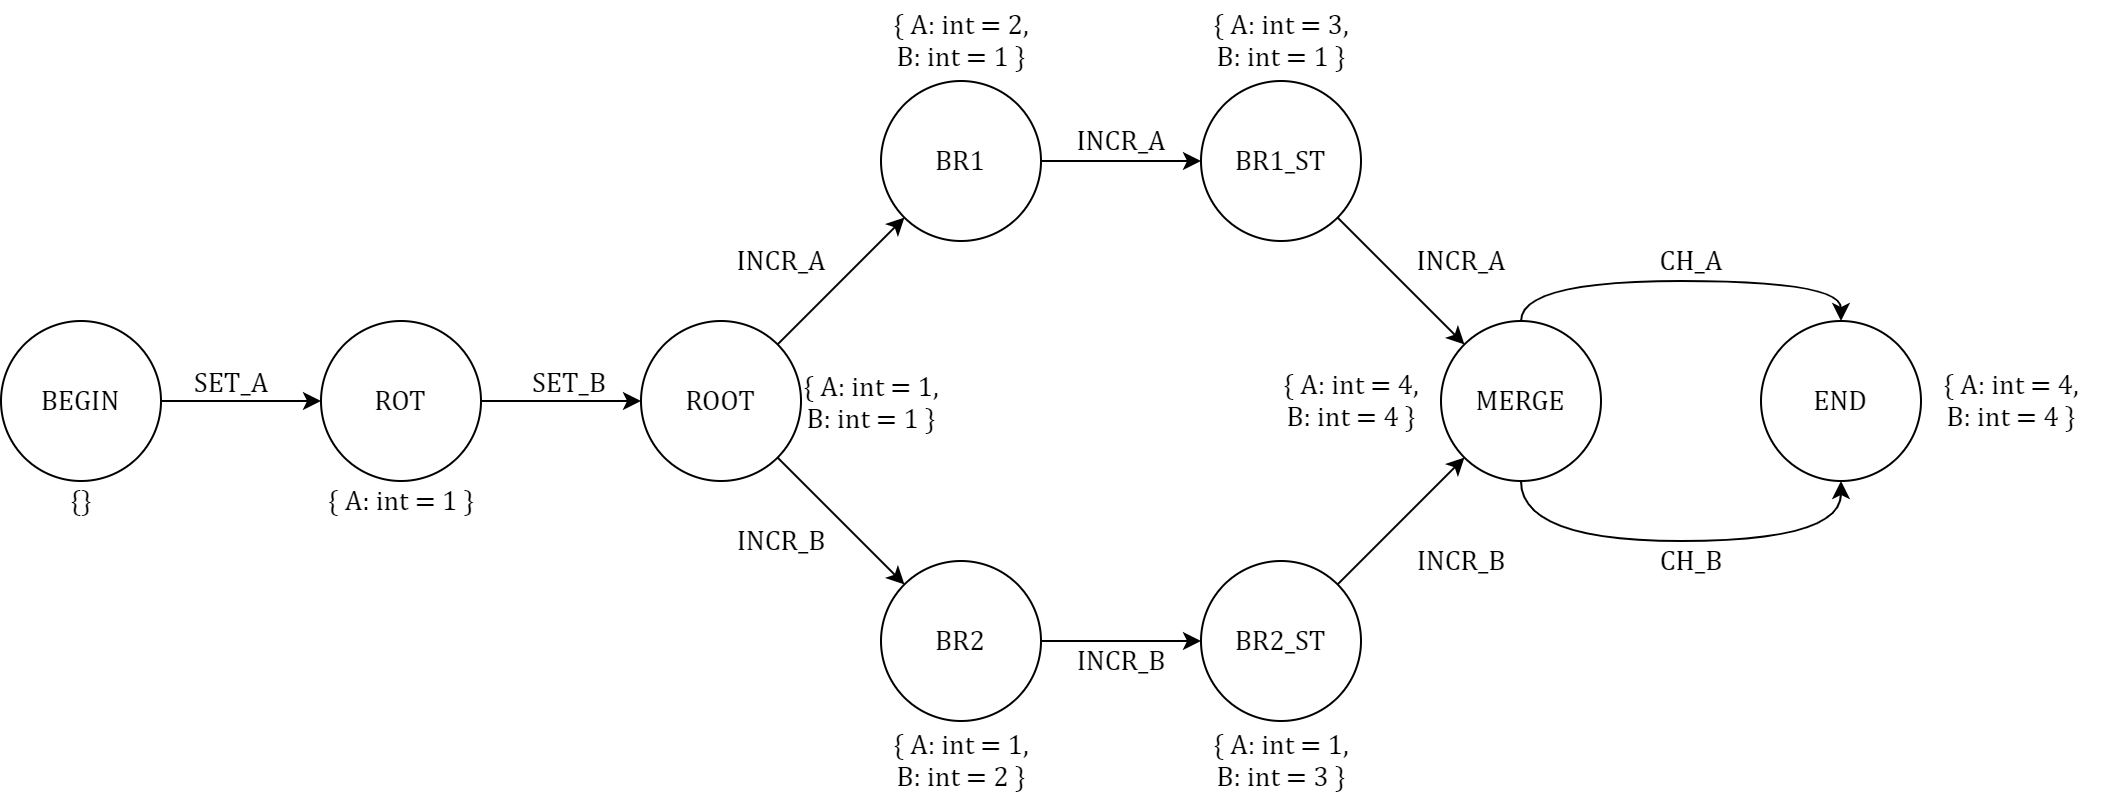
\includegraphics[width=\textwidth]{images/adot_example.png}
    \caption{Пример графовой модели вычислительного процесса}\label{fig:aDotExamplePic}
  \end{figure}
\end{frame}

\begin{frame}
%  Дополнительные определения:
  \begin{designation}
    \emph{Функция-обработчик} -- функция, осуществляющая преобразование данных из одного состояния в другое.    
  \end{designation}
  \begin{designation}
    \emph{Функция-предикат} -- функция, проверяющая корректность входного набора данных, соответствие их входному состоянию.
  \end{designation}
  \begin{designation}
    \emph{Функция-селектор} -- функция, отвечающая в процессе обхода графовой модели за выбор тех рёбер, которые необходимо выполнить на следующем шаге в соответствии с некоторым условием.    
  \end{designation}
\end{frame}

\begin{frame}
  \begin{remark}
    Функции-селекторы реализуют условное выполнение ветвей графовой модели.
  \end{remark}
  \begin{remark}
    Рёбра, относящиеся к разным ветвям графовой модели могут быть выполнены параллельно.
  \end{remark}
  \begin{figure}
    \centering
    \includegraphics[height=0.4\textheight]{images/new_structure_example.png}
    \caption{Пример графовой модели с использованием селекторов}
  \end{figure}
\end{frame}